% !TEX program = pdfLaTeX
\documentclass{scrartcl}
\usepackage[utf8]{inputenc}
\usepackage[T1]{fontenc} 
\usepackage[bitstream-charter]{mathdesign}
\usepackage[english]{babel}
\usepackage{fetamont,url,tikz,verbatim,listings,inconsolata,amsmath,microtype}
\usetikzlibrary{positioning}
\setkomafont{sectioning}{\rmfamily\bfseries\boldmath}
\renewcommand{\descriptionlabel}[1]{\hspace{\labelsep}\texttt{#1}}
\title{mf2outline}
\author{Linus Romer}

\lstset{basicstyle=\scriptsize\ttfamily,breaklines=true}

\begin{document}	
%
\maketitle
%
\tableofcontents
%
\section{Introduction}
%
\MF{} is a very versatile font description language, especially when you need to design several faces of a typeface family. However, the \MF{} compiler has some severe restrictions:
\begin{itemize}
	\item The \MF{} compiler can only produce bitmaps and cannot produce outline font formats like Type~1 or OpenType.
	\item The \MF{} compiler cannot write more than 256 different characters per font.
\end{itemize}
Luckily, the \MP{} language and its compiler (see \cite{hobby13}) can be used as an expediant. Together with the \verb|mfplain.mp| base, the \MP{} language supersets nearly 100~\% of the \MF{} language. The \MP{} compiler outputs PostScript files, which can be imported in FontForge and then be converted to outline font formats. This process is automated by the \verb|mf2outline.py| script. 

For compatiblity reasons, the \verb|mfplain.mp| base does not support more than 256 different characters per font. To get over this and other artificial restriction, the \verb|mf2outline.mp| base extends the capabilities of the \verb|mfplain.mp| base. Of course, the backwards compatibility to \MF{} will be lost by using these extensions.

\begin{center}
	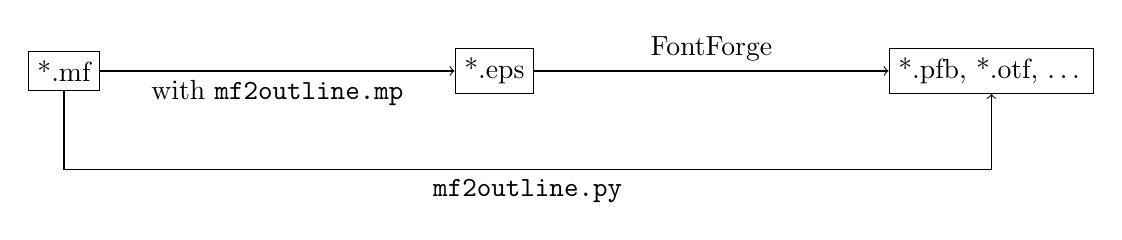
\begin{tikzpicture}[node distance=4.5cm]  
		\node[rectangle,draw](mf){*.mf};
		\node[rectangle,draw,right=of mf](eps){*.eps};
		\node[rectangle,draw,right=of eps](pfb){*.pfb, *.otf, \ldots};
		\draw[->] (mf.east) -- (eps.west) node[pos=.5,above]{\MP} node[pos=.5,below]{with \verb|mf2outline.mp|};
		\draw[->] (eps.east) -- (pfb.west) node[pos=.5,above]{FontForge};
		\draw[->] (mf.south) -- ++(0,-1) -| (pfb.south) node[pos=.25,below]{\verb|mf2outline.py|};
	\end{tikzpicture}
\end{center}
%
\section{The \texttt{mf2outline.py} Script}
%
\subsection{Requirements}
%
The following programs have to be installed before using \verb|mf2outline|:
%
\begin{itemize}
	\item Python interpreter (\verb|mf2outline.py| is a Python script)
	\item \MP{} compiler
	\item FontForge's python extension (\verb|python-fontforge|)
	\item (minimal) \LaTeX{} (for pdf proofs only)
\end{itemize}
%
\subsection{Usage and Command-line Options}
%
The general usage for a \MF{} file \verb|mfsource| is easy:
\begin{verbatim}
	mf2outline.py mfsource
\end{verbatim}
%
This will output an OpenType font file named \verb|mfsource.otf| in your working directory. The file extension \verb|.mf| of the specified \MF{} source file can be omitted.

You may add some of these optional arguments:
\begin{description}
	\item[-h, -{}-help] \hfill \\
		Show the help message and exit.
	\item[-v, -{}-verbose ] \hfill \\
		Explain what is being done.\\
		Default: False
	\item[-vv, -{}-veryverbose] \hfill \\
		Explain very detailed what is being done.\\
		Default: False
	\item[-{}-designsize SIZE] \hfill \\
		Force the designsize to be SIZE (e.g. 12 for 12pt).\\
		Default: 10pt at first guess, but if the 
		designsize is defined somewhere in the mf sources,
		a new run with the correct size will be launched.
	\item[-{}-raw] \hfill \\
		Do not remove overlaps, round to int, add extrema, add hints\ldots\\
		Default: False
	\item[-{}-ignore-tfm] \hfill \\
		Do not read any data from the tfm file...\ldots\\
		Default: False
	\item[-{}-max256] \hfill \\	
		Use charcode (256 codes) instead of charunicode
		(1111998 codes). This is needed for Malvern Greek.\\
		Default: False
	\item[-{}-preview] \hfill \\
		Use icosagon pens instead of circle/elliptic pens and do not 
		care about advanced font features like kerning and ligatures 
		(makes things faster, mainly used for \textffm{METAFLOP}).\\
		Default: False
	\item[-{}-use-ff-commands] \hfill \\
		Read additional fontforge commands from mf2outline.txt.
		This may be insecure (uses exec)...\\
		Default: False
	\item[-f FORMATS, -{}-formats FORMATS] \hfill \\
		Generate the formats FORMATS (comma separated list).\\
		Supported formats: sfd, afm, pfa, pfb, otf, ttf, eoff, 
		svg, tfm, pdf (proof).\\
		Default: otf
	\item[-{}-encoding ENC ] \hfill \\
		Force the font encoding to be ENC.\\
		Natively supported encodings: ot1, t1, unicode\\
		Default: unicode\\
		The file ENC.enc will be read if it exists in the same directory as the source file (the encoding name inside the encoding file must be named ENC, too).
	\item[-{}-fullname FULL] \hfill \\
		Set the full name to FULL (with modifiers and possible spaces).
	\item[-{}-fontname NAME] \hfill \\
		Set the font name to NAME (with modifiers and without spaces).
	\item[-{}-familyname FAM] \hfill \\
		Set the font family name to FAM.
	\item[-{}-fullname-as-filename] \hfill \\
		Use the fullname for the name of the output file.
	\item[-{}-fontversion VERS] \hfill \\
		Set the version of the font to VERS.\\
		Default: 001.001
	\item[-{}-copyright COPY] \hfill \\
		Set the copyright notice of the font to COPY.
	\item[-{}-vendor VEND] \hfill \\
		Set the vendor name of the font to VEND (limited to 4 characters).
	\item[-{}-weight WGT] \hfill \\
		 Force the OS/2 weight of the font to be WGT.\\
		 The weight number is mapped to the following PostScript weight names:
		 \begin{itemize}
		 	\item[100] Thin
		 	\item[200] Extra-Light
		 	\item[300] Light
		 	\item[400] Book
		 	\item[500] Medium 
		 	\item[600] Demi-Bold
		 	\item[700] Bold
		 	\item[800] Heavy
		 	\item[900] Black
		 \end{itemize}
	\item[-{}-width WDT] \hfill \\
		Force the OS/2 width of the font to be WDT.\\
		 The width number stands for the following width names:
		 \begin{itemize}
		 	\item[1] Ultra-condensed
		 	\item[2] Extra-condensed
		 	\item[3] Condensed
		 	\item[4] Semi-condensed
		 	\item[5] Medium (normal)
		 	\item[6] Semi-expanded
		 	\item[7] Expanded
		 	\item[8] Extra-expanded
		 	\item[9] Ultra-expanded
		 \end{itemize}
	\item[ -{}-ffscript FFSCRIPT] \hfill \\
		Specify an own finetuning fontforge script (e.g. finetune.pe). The script file has to be in the same directory as the source file. Example script:\\
		\verb|Open($1);|\\
		\verb|SelectAll();|\\
		\verb|RemoveOverlap();|\\
		\verb|Generate($1);|\\
		\verb|Quit(0);|
\end{description}
%
\subsection{Restrictions}
%
Not every valid \MF{} typeface can be automatically converted by \verb|mf2outline|. The three most important restrictions are listed below:
\begin{itemize}
	\item The \MF{} typeface cannot be compiled by \MP{} when it uses some special features of \MF{} that are not implemented in \MP{} (e.g. \emph{Pandora}).
	\item If the font uses many overlapping filldrawn areas, FontForge does not always import the PostScript files correctly (e.g. Computer Modern). As a solution, you can use the \verb|--raw| option and finetune the font by hand in FontForge.
	\item As a mathematical fact, a generic cubic beziér spline path that is drawn by a elliptic pen cannot be converted perfectly to cubic beziér spline outlines. Hence, FontForge does only an approximation job here. This approximation is normally very close to the original shape, but if you use heavily twisted cubic beziér splines, the approximation will be unsatisfactory.
\end{itemize}
%
\subsection{\textffm{METAFLOP}}
%
\textffm{METAFLOP} is an easy to use web application for modulating \MF{} fonts:
\begin{center}
	\url{http://www.metaflop.com/modulator}
\end{center}
The conversion to outline formats is being done by \verb|mf2outline|. 
%
\subsection{Other Tools}
%
The following two programs are alternatives to \verb|mf2outline|.
%
\begin{description}
	\item[mftrace] is a python script that converts \MF{} fonts into Type~1 fonts. Unlike \verb|mf2outline|, \verb|mftrace| can cope with \emph{every} valid \MF{} font. Unfortunately, the outline paths are not that neat.
	\item[mf2pt1] is a perl script that converts \MF{} fonts into Type~1 fonts. Actually, \verb|mf2pt1| is pretty similar to \verb|mf2outline|, but does not rely that much on FontForge.
\end{description}
%
Both programs, \verb|mftrace| and \verb|mf2pt1|, have deeply inspired the author of \verb|mf2outline|. Thus, many ideas of the two programs can be found in \verb|mf2outline|, too.
%
\section{Example Use Of \texttt{mf2outline} Extensions}
%
The following example will show an example \MF{} file, that uses the \texttt{mf2outline} extensions. Remember: The backwards compatibility to the \MF{} compiler to these extensions is not given! 
\lstset{columns=fullflexible}
\begin{lstlisting}
font_familyname "Quindesch";
font_name "Quindesch-Regular10";
font_fullname "Quindesch Regular 10";
font_identifier "FQDR";
font_copyright "Linus Romer, 2015";
font_version "1.000";
font_coding_scheme "Unicode";
font_size 10pt#;                     % the "design size" of this font 
font_slant 0;                        % general slanting of the font   
font_normal_space .23designsize;
font_normal_stretch .12designsize;
font_normal_shrink .08designsize;
font_x_height .435designsize;
font_quad .69designsize;
font_normal_shrink .08designsize;
font_os_weight 400;                  % weight 400 means regular, 700 means bold
font_os_width 5;                     % width 5 means regular, 3 means condensed

% ... (definitions of font variables and glyphs) ...

fontforge("font.addLookup('ligatures','gsub_ligature',(),(('liga',(('latn',('dflt')),)),))");
fontforge("font.addLookupSubtable('ligatures','ligatures subtable')");
fontforge("font['uniFB00'].addPosSub('ligatures subtable',('f','f'))");
fontforge("font.addLookup('kerning','gpos_pair',(),(('kern',(('latn',('dflt')),)),))");
fontforge("font.addLookupSubtable('kerning','kerning subtable')");
fontforge("font['A'].addPosSub('kerning subtable','V',-100)");
\end{lstlisting}
%
\section{The \texttt{mf2outline.mp} Base}
%
\subsection{Unicode Support}
%
\MF{} can pack at most $2^{8}=256$ glyphs in a font. \MP{} can output nearly arbitrary many PostScript files (each containing one glyph). For compatibility reasons, \MP{} combined with \texttt{mfplain.mp} restricts the glyph code $c$ to be a byte (which is a number between $0$ to $255$):
\lstset{language=MetaPost,columns=fullflexible}
\begin{lstlisting}
def beginchar(expr c,w_sharp,h_sharp,d_sharp) =
 begingroup
 charcode:=if known c: byte c else: 0 fi;
 charwd:=w_sharp;      charht:=h_sharp;       chardp:=d_sharp;
 w:=charwd*pt; h:=charht*pt; d:=chardp*pt;
 charic:=0; clearxy; clearit; clearpen; scantokens extra_beginchar;
 enddef;
\end{lstlisting}
%
Another restriction is common to both, \MF{} and \MP: Numbers are represented in fixed point arithmetic as integer multiples of $2^{-16}$ and can (normally) not be greater than $4096=2^{12}$. Unicode contains 17 planes of $2^{16}$ glyphs with a code range from 000000 to 10FFFF. In \texttt{mfplain}, these hexadecimal unicode codes are represented by a string of length $6$ or a two byte number \emph{charext} and a one byte number \emph{charcode}. Thus, the code of the letter «J» can be represented in the following variants:
\[
	\underbrace{74}_{\text{decimal}}\quad=\quad\underbrace{\text{"00004A"}}_{\text{string}}\quad=\;\underbrace{\binom{\mathrm{hex}(\text{"0000"})}{\mathrm{hex}(\text{"4A"})}}_{\text{charext/charcode}}\quad=\;\underbrace{\binom{0}{74}}_{\text{charext/charcode}}
\]
The \texttt{beginchar} macro in \texttt{mf2outline.mp} is redefined as follows:
\lstset{language=MetaPost,columns=fullflexible}
\begin{lstlisting}
newinternal string charunicode;
def beginchar(expr c,w_sharp,h_sharp,d_sharp) =
  begingroup
    charunicode:=if known c: unicode c else: "0000" fi; 
    charcode:=hex(substring(2,4) of charunicode); 
    charext:=hex(substring(0,2) of charunicode); 
    charwd:=w_sharp;      charht:=h_sharp;       chardp:=d_sharp;
    w:=charwd*pt; h:=charht*pt; d:=chardp*pt;
    charic:=0; clearxy; clearit; clearpen; scantokens extra_beginchar;
enddef;
\end{lstlisting}
%
There are two additional macros necessary:
\begin{itemize}
	\item \texttt{hexadecimal} converts a decimal number to a hexadecimal string, e.g. hexadecimal(74) =~"4A".
	\item \texttt{unicode} converts a decimal number or a string to a hexadecimal string of length 4, e.g. unicode(74) =~unicode("J") =~unicode("004A") ~="004A".
\end{itemize}
%
The \texttt{hexadecimal} macro is defined as follows:
%
\lstset{language=MetaPost,columns=fullflexible}
\begin{lstlisting}
vardef hexadecimal primary n =
 save m,s;
 m:=abs round n; 
 string s; 
 s=
 if (m mod 16)<10:
  decimal(m mod 16)
 elseif (m mod 16)=10:
  "A"
 elseif (m mod 16)=11:
  "B"
 elseif (m mod 16)=12:
  "C"
 elseif (m mod 16)=13:
  "D"
 elseif (m mod 16)=14:
  "E"
 else:
  "F"
 fi
 ;
 forever:
  m:=m div 16; 
  exitif m=0;
  s:=
  if (m mod 16)<10:
   decimal(m mod 16)
  elseif (m mod 16)=10:
   "A"
  elseif (m mod 16)=11:
   "B"
  elseif (m mod 16)=12:
   "C"
  elseif (m mod 16)=13:
   "D"
  elseif (m mod 16)=14:
   "E"
  else:
   "F"
  fi
  & s; 
 endfor
 s
enddef;
\end{lstlisting}
%
The \texttt{unicode} macro is defined as follows:\\
!!!!!!!!!!!!!NEEDS UPDATE (IS NOW FILLED TO 6 DIGITS)

!!!!!!!!!!!!!NEEDS UPDATE (epscode)

!!!!!!!!!!!!!NEEDS UPDATE (epstounicode)
%
\lstset{language=MetaPost,columns=fullflexible}
\begin{lstlisting}
vardef unicode primary n = 
 save s,z;
 string s,z;
 s:=
 if string n:
  if length(n)=1: % assume n to be a glyph name like "W"
   hexadecimal(ASCII n);
  else: % assume n to be a unicode like "004A" (or even "4A")
   n;
  fi
 else: % assume n to be a numeric 
  hexadecimal n;
 fi 
 % now fill zeroes to be a 4-digit word:
 z:=
 if length(s)<4:
  for i=1 upto (4-length(s)): "0" & endfor s;
 else:
  s;
 fi
 z
enddef;
\end{lstlisting}
%
\subsection{Additional Font and Glyph Parameters}
%
Unlike \texttt{mfplain.mp}, the \texttt{mf2outline.mp} base forces \MP{} to write special additional glyph information to the PostScript files and to generate an additional file mf2outline.txt, that contains general font information. Normally, some of these additional information are stored in the \texttt{tfm} file.
%
\subsubsection{The Old Way --- TFM}
%
The \texttt{tfm} file stores amongst other things the following parameters:
\begin{itemize}
	\item Global font parameters:
	\begin{itemize}
		\item font\_size
		\item font\_slant
		\item font\_normal\_space
		\item font\_normal\_stretch
		\item font\_normal\_shrink
		\item font\_x\_height
		\item font\_quad
		\item font\_extra\_space
		\item font\_identifier (normally not stored)
		\item font\_coding\_scheme (normally not stored)
	\end{itemize}
	\item Glyph parameters:
	\begin{itemize}
		\item charwd (character width)
		\item charht (character height)
		\item chardp (character depth)
		\item charic (character italic correction)
		\item charcode (code number of the character)
		\item charext (code extension number of the character)
		\item chardx (horizontal escapement of glyph positioning)
		\item chardy (vertical escapement of glyph positioning)
	\end{itemize}
\end{itemize}
%
\subsubsection{The New Way --- \texttt{mf2outline.txt} \& PostScript Comments}
%
The \texttt{mf2outline.mp} base defines some new parameters that cannot be stored in the \texttt{tfm} format:
\begin{itemize}
	\item Global font parameters:
	\begin{itemize}
		\item font\_os\_weight
		\item font\_os\_width
		\item font\_version
		\item font\_copyright
		\item font\_name
		\item font\_fullname
		\item font\_familyname
	\end{itemize}
	\item Glyph parameters:
	\begin{itemize}
		\item charunicode (unicode string like \verb|"004A"|)
	\end{itemize}
\end{itemize}
%
\subsection{Kerning and Ligatures}
%
If one want to kern the pair «AV» in \MF{} one needs an instruction like
\lstset{language=MetaPost,columns=fullflexible}
\begin{lstlisting}
ligtable "A": "V" kern -u#;
\end{lstlisting}
However, \texttt{ligtable} cannot handle unicode characters nor kerning classes. Use fontforge macros inside the \verb|fontforge()| command. These macros work like their corresponding python functions of python-fontforge described in \cite{williams15}.
!!!!!!!!!!!!!NEEDS UPDATE (KERNING AND LIGATURES AND SIZE RANGE WILL BE SUPPORTED)
%
\subsection{Writing Temporary Text Files}
%
All the global font parameters, kerning, position and substitution data are written to \texttt{mf2outline.txt}, whereas all glyph parameters are appended to the glyph PostScript files.
%
\begin{thebibliography}{Williams15}
	\bibitem[Williams15]{williams15}
	George Williams
	\emph{Writing python scripts to change fonts in FontForge}.
	\url{fontforge.github.io/python.html}, 2015
	\bibitem[Hobby13]{hobby13}
	John D. Hobby et al.
	\emph{\MP{} -- A User's Manual}.
	\url{www.tug.org/docs/metapost/mpman.pdf}, 2013
\end{thebibliography}

\end{document}
